%%%%%%%%%%%%%%%%%%%%%%%%%%%%%%%%%%%%%%%%%%%%%%%%%%%%%%%%%%%%%%%%%%%%%%%%%%%%%%%%%%%%%%%%%%%%%%%%%%%
%%%%%%%%%%%%%%%%%%%%%%%%%%%%%%%%%%%%%%%%%%%%%%%%%%%%%%%%%%%%%%%%%%%%%%%%%%%%%%%%%%%%%%%%%%%%%%%%%%%
%%%%%%%%%%%%%%%%%%%%%%%%%%%%%%%%%%%%%%%%%%%%%%%%%%%%%%%%%%%%%%%%%%%%%%%%%%%%%%%%%%%%%%%%%%%%%%%%%%%
%%%%%%%%%%%%%%%%%%%%%%%%%%%%%%%%%%%%%%%%%%%%%%%%%%%%%%%%%%%%%%%%%%%%%%%%%%%%%%%%%%%%%%%%%%%%%%%%%%%
\chapter{Metodología}

%El presente trabajo resulta de una colaboración con el departamento de Gerontología, dependiente 
%del Instituto de Ciencias de la Salud (ICSA); parte de esta colaboración incluye el acceso a los 
%registros de PSG obtenidos por Vázquez Tagle y colaboradores \cite{VazquezTagle16}. 
%A continuación se expone la metodología de aquél estudio.

\section{Participantes}

Los sujetos fueron elegidos usando un muestreo \textit{no probabilístico por 
conveniencia}\footnote{Lo cual implica que los resultados pueden no deben ser interpolados 
inmediatamente a poblaciones más grandes} bajo los siguientes criterios de inclusión:
\begin{itemize}
\item Edad entre 60 y 85 años
\item Diestros (mano derecha dominante)
\item Sin ansiedad, depresión ni síndromes focales
\item No usar medicamentos o sustancias para dormir
\item Firma de consentimiento informado
\item Voluntario para el registro de PSG
\end{itemize}

Un total de 14 adultos mayores cumplieron los criterios de inclusión. Estos 
participantes fueron 
sometidos a una batería de pruebas neuropsicológicas para determinar su estado cognoscitivo general 
(Neuropsi, MMSE), descartar cuadros depresivos (GDS, SATS) y cambios en la vida cotidiana (KATZ).
En base a las pruebas se determinó que, objetivamente, 9 de los voluntarios no padecen depresión ni 
ansiedad, además de que no presentan afectaciones significativas en la vida diaria.

Para su análisis, los 9 participantes se dividieron en dos grupos en base a su estado cognoscitivo:
control (CTL) y con Probable Deterioro Cognitivo (PDC). 
Para esta clasificación se dio mayor atención al puntaje de Neuropsi, estandarizado 
según edad y escolaridad (tabla \ref{puntajes}). Al puntaje de MMSE se le otorgó menos importancia
como clasificador debido a que tiene baja sensibilidad para el diagnóstico de deterioro cognitivo 
leve \cite{Ardila12}, y baja especificidad\footnote{Especificidad es 
la probabilidad de que un individuo sano obtenga un resultado negativo en la prueba de deterioro 
cognitivo} para individuos con escolaridad muy baja o muy alta \cite{Ostrosky00}, una situación 
presente en los adultos mayores participantes.

%Para la clasificación se dio especial 
%atención al puntaje total de Neuropsi estandarizado según edad y escolaridad \cite{Ardila12}, 
%criterios que se muestran en la tabla \ref{puntajes}.

\begin{table}
\centering
\caption{Puntajes de corte para la prueba Neuropsi}
\begin{tabular}{llccrccc}
\toprule
&& \multicolumn{2}{l}{Sano} & \phantom{.} & \multicolumn{3}{l}{Deterioro cognitivo} \\
\cmidrule{3-4} \cmidrule{6-8} 
Escolaridad & Edad & Alto & Normal && Leve & Moderado & Severo\\
\midrule
Nula
& 16 -- 30 &\ppu 92 &\ppu 60 &&\ppu 45 & 30 & 14 \\
& 31 -- 50 &\ppu 95 &\ppu 68 &&\ppu 54 & 41 & 28 \\
& 51 -- 65 &\ppu 91 &\ppu 59 &&\ppu 44 & 28 & 13 \\
& 66 -- 85 &\ppu 76 &\ppu 48 &&\ppu 34 & 20 &\ppu 6 \\
\midrule
1 -- 4 años
& 16 -- 30 &    105 &\ppu 73 &&\ppu 58 & 42 & 27 \\
& 31 -- 50 &    105 &\ppu 81 &&\ppu 69 & 58 & 46 \\
& 51 -- 65 &\ppu 98 &\ppu 77 &&\ppu 67 & 57 & 47 \\
& 66 -- 85 &\ppu 90 &\ppu 61 &&\ppu 46 & 32 & 18 \\
\midrule
5 -- 9 años
& 16 -- 30 &    114 &    102 &&\ppu 97 & 86 & 75 \\
& 31 -- 50 &    118 &    106 &&    101 & 90 & 79 \\
& 51 -- 65 &    111 &\ppu 98 &&\ppu 91 & 79 & 67 \\
& 66 -- 85 &\ppu 97 &\ppu 80 &&\ppu 72 & 56 & 39 \\
\midrule
10 -- 24 años
& 16 -- 30 &    115 &    103 &&\ppu 98 & 87 & 77 \\
& 31 -- 50 &    113 &    102 &&\ppu 97 & 88 & 78 \\
& 51 -- 65 &    102 &\ppu 93 &&\ppu 88 & 80 & 72 \\
& 66 -- 85 &\ppu 92 &\ppu 78 &&\ppu 72 & 59 & 46 \\
\bottomrule
\multicolumn{5}{l}{Fuente: Ardila y Ostrosky \cite{Ardila12}}
\end{tabular}
\label{puntajes}
\end{table}

%\begin{table}[h]
%\centering
%\begin{tabular}{lcl}
%\toprule
%Grupo & Sujetos & Características \\
%\midrule
%Mn & 4 & Posible Deterioro Cognitivo \\
%Nn & 5 & Sin PDC \\
%ex & 3 & No satisfacen los criterios de inclusión \\
%\bottomrule
%\end{tabular}
%\end{table}

%El grupo ex se conforma de sujeto que incumplen al menos uno de los criterios de inclusión: {FGH} 
%padece parálisis facial y posiblemente daño cerebral (síndromes focales), MGG padece depresión, 
%EMT no califica como adulto mayor por su edad.
%Se efectuaron todos los análisis sobre este grupo, con la finalidad de exhibir las capacidades y
%limitaciones de las técnicas utilizadas; por ello este grupo es ignorado en la sección de 
%resultados pero no en la discusión.

\begin{table}
\caption{Datos generales de los participantes}
\centering
\bordes{1.1}
{\small
\begin{tabular}{llcrrrrrrr}
\toprule
 \phantom{.}&
 & {Sexo} & {Edad} & {Escol.} & {Neuropsi} & {MMSE} & {SATS} & {KATZ} & {GDS} \\
\midrule
\multicolumn{6}{l}{\textbf{Grupo CTL}}\\
&VCR    & F    & 59\pz & 12\pz & 107\pz & 29\pz & 21\pz & 0\pz & 3\pz \\
&MJH    & F    & 72\pz & 9\pz  & 113\pz & 30\pz & 18\pz & 0\pz & 0\pz \\
&JAE    & F    & 78\pz & 5\pz  & 102\pz & 28\pz & 19\pz & 0\pz & 5\pz \\
&GHA    & M    & 65\pz & 9\pz  & 107.5  & 30\pz & 23\pz & 0\pz & 7\pz \\
&MFGR   & F    & 67\pz & 11\pz & 115\pz & 30\pz & 18\pz & 0\pz &      \\
\rowcolor{gris}
&\multicolumn{1}{c}{$\widehat{\mu}$} & 
               & 68.2  & 9.2   & 108.9  & 29.4  & 19.8  & 0.0  & 3.0  \\
\rowcolor{gris}
&\multicolumn{1}{c}{$\widehat{\sigma}$} & 
               & 7.2   & 2.7   & 5.2    & 0.9   & 2.2   & 0.0  & 3.0  \\
\midrulec
%\hline
\multicolumn{6}{l}{\textbf{Grupo PDC}}\\
&CLO    & F    & 68\pz & 5\pz  & 81\pz & 28\pz & 22\pz & 1\pz & 6\pz \\
&RLO    & F    & 63\pz & 9\pz  & 90\pz & 29\pz & 20\pz & 0\pz & 3\pz \\
&RRU    & M    & 69\pz & 9\pz  & 85\pz & 27\pz & 10\pz & 0\pz & 3\pz \\
&JGZ    & M    & 65\pz & 11\pz & 87\pz & 25\pz & 20\pz & 0\pz & 1\pz \\
%\rowcolor{gris}
%&\multicolumn{1}{c}{$\widehat{\mu}$} & 
%              & 66.3   & 8.5   & 85.8  & 27.3  & 18.0  & 0.3  & 3.3  \\
%\rowcolor{gris}
%&\multicolumn{1}{c}{$\widehat{\sigma}$} & 
%              & 2.8    & 2.5   & 3.8   & 1.7   & 5.4   & 0.5  & 2.1  \\
&AEFP   & M    & 73\pz &  8\pz & 96\pz & 29\pz &   \pz & 0\pz & 2\pz \\
\rowcolor{gris}
&\multicolumn{1}{c}{$\widehat{\mu}$} & 
              & 67.6   & 8.4   & 87.8  & 27.4  & 18.0  & 0.2  & 3.0  \\
\rowcolor{gris}
&\multicolumn{1}{c}{$\widehat{\sigma}$} & 
              & 3.4    & 2.2   & 5.6   & 1.8   & 5.4   & 0.4  & 1.9  \\
\bottomrulec
\end{tabular} 
}
\label{tab_sujetos}
\end{table}

%\begin{table}
%\centering
%\bordes{1.1}
%\begin{tabular}{c}
%\textbf{Datos generales de los participantes}
%\vspace{1em}
%\end{tabular}
%{\small
%\begin{tabular}{llcrrrrrrr}
%\toprule
% \phantom{.}&
% & {Sexo} & {Edad} & {Escol.} & {Neuropsi} & {MMSE} & {SATS} & {KATZ} & {Gds} \\
%\midrule
%\multicolumn{6}{l}{{Grupo Nn}}\\
%&VCR    & F    & 59\pz & 12\pz & 107\pz & 29\pz & 21\pz & 0\pz & 3\pz \\
%&MJH    & F    & 72\pz & 9\pz  & 113\pz & 30\pz & 18\pz & 0\pz & 0\pz \\
%&JAE    & F    & 78\pz & 5\pz  & 102\pz & 28\pz & 19\pz & 0\pz & 5\pz \\
%&GHA    & M    & 65\pz & 9\pz  & 107.5  & 30\pz & 23\pz & 0\pz & 7\pz \\
%&MFGR   & F    & 67\pz & 11\pz & 110\pz & 30\pz & 18\pz & 0\pz &      \\
%\rowcolor{gris}
%&\multicolumn{1}{c}{$\widehat{\mu}$} & 
%               & 68.2  & 9.2   & 107.9  & 29.4  & 19.8  & 0.0  & 3.0  \\
%\rowcolor{gris}
%&\multicolumn{1}{c}{$\widehat{\sigma}$} & 
%               & 7.2   & 2.7   & 4.1    & 0.9   & 2.2   & 0.0  & 3.0  \\
%\midrulec
%%\hline
%\multicolumn{6}{l}{{Grupo Mn}}\\
%&CLO    & F    & 68\pz & 5\pz  & 81\pz & 28\pz & 22\pz & 1\pz & 6\pz \\
%&RLO    & F    & 63\pz & 9\pz  & 90\pz & 29\pz & 20\pz & 0\pz & 3\pz \\
%&RRU    & M    & 69\pz & 9\pz  & 85\pz & 27\pz & 10\pz & 0\pz & 3\pz \\
%&JGZ    & M    & 65\pz & 11\pz & 87\pz & 25\pz & 20\pz & 0\pz & 1\pz \\
%\rowcolor{gris}
%&\multicolumn{1}{c}{$\widehat{\mu}$} & 
%              & 66.3   & 8.5   & 85.8  & 27.3  & 18.0  & 0.3  & 3.3  \\
%\rowcolor{gris}
%&\multicolumn{1}{c}{$\widehat{\sigma}$} & 
%              & 2.8    & 2.5   & 3.8   & 1.7   & 5.4   & 0.5  & 2.1  \\
%\midrulec
%%\hline
%\multicolumn{6}{l}{{Grupo ex}}\\
%&FGH    & M    & 71\pz   & 9\pz    & 83.5     & 21\pz   & 23\pz   & 0\pz    & 4\pz  \\
%&MGG    & F    & 61\pz   & 9\pz    & 114\pz      & 28\pz   & 29\pz   & 1\pz    & 14\pz \\
%&EMT    & M    & 50\pz   & 22\pz   & 106\pz      & 30\pz   & 15\pz   & 0\pz    & 4\pz  \\
%\bottomrule
%\end{tabular} 
%}
%\label{tab_sujetos}
%\caption{Resultados de las pruebas neuropsicológicas 
%}
%\end{table}

%%%%%%%%%%%%%%%%%%%%%%%%%%%%%%%%%%%%%%%%%%%%%%%%%%%%%%%%%%%%%%%%%%%%%%%%%%%%%%%%%%%%%%%%%%%%%%%%%%%
%%%%%%%%%%%%%%%%%%%%%%%%%%%%%%%%%%%%%%%%%%%%%%%%%%%%%%%%%%%%%%%%%%%%%%%%%%%%%%%%%%%%%%%%%%%%%%%%%%%

\section{Registro del polisomnograma}

Para llevar a cabo el registro, los adultos mayores participantes fueron invitados a acudir a las 
instalaciones de la Clínica Gerontológica de Sueño, ubicada dentro del Instituto de Ciencias de la 
Salud (ICSa) dependiente de la Universidad Autónoma del Estado de Hidalgo. Los participantes 
recibieron instrucciones de realizar una rutina normal de actividades durante la semana que 
precedió al estudio, y se les recomendó no ingerir bebidas alcohólicas o energizantes (como café 
o refresco) durante las 24 horas previas al experimento, y que no durmieran siesta ese día.

Para efectuar el registro se usó un polisomnógrafo Medicid 5 (Neuronic Mexicana). El protocolo de 
PSG incluye 
\begin{itemize}
\item 19 electrodos de EEG, colocadas siguiendo las coordenadas del Sistema Internacional 10--20
\item 4 electrodos de EOG para movimientos oculares horizontales y verticales
\item 2 electrodos de EMG colocados en los músculos submentonianos
\end{itemize}
%
Los electrodos para registro de EEG fueron montados usando los lóbulos oculares como referencia
común; se mantuvo por debajo de \SI{50}{\micro\ohm}.

Las señales fueron amplificadas analógicamente usando amplificadores de alta ganancia en cadena, 
y adicionalmente fueron filtradas analógicamente usando filtros de paso de banda: 0.1--100 Hz 
para EEG, 3--20 Hz para EOG. 
Debido a dificultades técnicas el registro se efectuó a razón de 512 puntos por segundo (Hz) para 
algunos participantes, mientras que se usó 200 Hz para otros; en ambos casos se cumple la 
recomendación de la AASM de al menos 128 Hz.
%
Los registros digitalizados fueron almacenados en formato de texto bajo la codificación 
ASCII.
%, mientras que en un archivo separado se indicaron las épocas clasificadas como de sueño MOR.

Los registros fueron segmentados en ventanas de 30 segundos de duración, referidas como 
\textit{épocas}, para su estudio posterior \textit{fuera de línea}. 
Usando los criterios de la AASM, cada una de las épocas fueron clasificadas según la etapa
de sueño como MOR o NMOR. Dicha clasificación fue llevada a cabo por expertos en sueño de ICSa.

%La clasificación del PSG en fases de sueño se realizó \textit{manualmente} sobre épocas de 30 
%segundos siguiendo los criterios estandarizados de la AASM.

%Debido a un cambio en el polisomnógrafo 
%usado, la frecuencia de muestreo (en Hz) cambia entre sujetos.



\begin{table}
\centering
\caption{Datos generales sobre los registros de PSG}
\bordes{1.2}
{\small
\begin{tabular}{llcllcllr}
\toprule
    \phantom{.}&
    &\multirow{2}{*}{\bordes{1}\begin{tabular}{l}Frecuencia de\\ muestreo [\hz]\end{tabular}}
    \bordes{1.2}
    & \multicolumn{2}{c}{Total} & \phantom{l}   & \multicolumn{3}{c}{MOR*}\\
    \cmidrule{4-5}  \cmidrule{7-9}
    &&          &Puntos  &  Tiempo   &&Puntos  &  Tiempo   &  \% \\
\midrule
\multicolumn{6}{l}{\textbf{Grupo CTL}}\\
&VCR &200       &\ppu 5166000 & \ppu  7:10:30 &&\ppu 438000 &   0:36:30 & 8.48 \\
&MJH &512       &    15851520 & \ppu  8:36:00 &&    1950720 &   1:03:30 &12.31 \\
&JAE &512       &    13931520 & \ppu  7:33:30 &&    2626560 &   1:25:30 &18.85 \\
&GHA &200       &\ppu 6558000 & \ppu  9:06:30 &&\ppu 330000 &   0:27:30 & 5.03 \\
&MFGR&200       &\ppu 4932000 & \ppu  6:51:00 &&\ppu 570000 &   0:47:30 &11.56 \\

\rowcolor{gris}
&\multicolumn{1}{c}{$\widehat{\mu}$}  
              & &        & \ppu 7:51:30   &&        &   0:52:06 &11.25 \\
\rowcolor{gris}
&\multicolumn{1}{c}{$\widehat{\sigma}$} 
              & &        & \ppu 0:57:36   &&        &   0:23:00 & 5.13 \\
\midrulec

\multicolumn{6}{l}{\textbf{Grupo PDC}}\\
&CLO &512       &    14499840 & \ppu  7:52:00 &&    2027520 &   1:06:00 &13.98 \\
&RLO &512       &    12994560 & \ppu  7:03:00 &&    1520640 &   0:49:30 &11.70 \\
&RRU &200       &\ppu 2484000 & \ppu  3:27:00 &&\ppu 228000 &   0:19:00 & 9.18 \\
&JGZ &512       &    18539520 &      10:03:30 &&\ppu 506880 &   0:16:30 & 2.73 \\
%\rowcolor{gris}
%&\multicolumn{1}{c}{$\widehat{\mu}$}  
%              & &        & \ppu 7:06:23   &&        &   0:37:45 &9.4 \\
%\rowcolor{gris}
%&\multicolumn{1}{c}{$\widehat{\sigma}$} 
%              & &        & \ppu 2:44:55   &&        &   0:24:05 &4.9 \\
&AEFP &512       &    14699520 &       7:58:30 &&\ppu 629760 &   0:20:30 & 4.28 \\

\rowcolor{gris}
&\multicolumn{1}{c}{$\widehat{\mu}$}  
              & &        & \ppu 7:16:48   &&        &   0:34:18 &8.38 \\
\rowcolor{gris}
&\multicolumn{1}{c}{$\widehat{\sigma}$} 
              & &        & \ppu 2:24:43   &&        &   0:22:14 &4.79 \\
\bottomrulec
\end{tabular}\\
*Dado que el sueño MOR aparece fragmentado, se reporta la suma de tales tiempos
}
\label{frecuencias}
\end{table}

%\begin{table}
%\centering
%\bordes{1.2}
%\begin{tabular}{c}
%\textbf{Datos generales sobre los registros de PSG}
%\vspace{1em}
%\end{tabular}
%{\small
%\begin{tabular}{llcrrcrrr}
%\toprule
%    \phantom{.}&
%    &\multirow{2}{*}{\bordes{1}\begin{tabular}{l}Frecuencia\\ muestreo\end{tabular}}
%    \bordes{1.2}
%    & \multicolumn{2}{c}{Total} & \phantom{l}   & \multicolumn{3}{c}{MOR*}\\
%    \cmidrule{4-5}  \cmidrule{7-9}
%    &&          &Puntos  &  Tiempo   &&Puntos  &  Tiempo   &  \% MOR \\
%\midrule
%\multicolumn{6}{l}{{Grupo Nn}}\\
%&VCR &200       & 5166000&   7:10:30 &&438000  &   0:36:30 & 8.5\% \\
%&MJH &512       &15851520&   8:36:00 &&1950720 &   1:03:30 &12.3\% \\
%&JAE &512       &13931520&   7:33:30 &&2626560 &   1:25:30 &18.9\% \\
%&GHA &200       &6558000 &   9:06:00 &&330000  &   0:27:30 & 5.0\% \\
%&MFGR&200       &4932000 &   6:51:00 &&570000  &   0:47:30 &11.6\% \\
%
%\rowcolor{gris}
%&\multicolumn{1}{c}{$\widehat{\mu}$}  
%              & &        & 7:51:30   &&        &   0:52:06 &11.2\% \\
%\rowcolor{gris}
%&\multicolumn{1}{c}{$\widehat{\sigma}$} 
%              & &        & 0:57:36   &&        &   0:23:00 & 5.1\% \\
%\midrulec
%
%\multicolumn{6}{l}{{Grupo Mn}}\\
%&CLO &512       &14499840&   7:52:00 &&2027520 &   1:06:00 &14.0\% \\
%&RLO &512       &12994560&   7:03:00 &&1520640 &   0:49:30 &11.7\% \\
%&RRU &200       &2484000 &   3:27:00 &&228000  &   0:19:00 & 9.2\% \\
%&JGZ &512       &18539520&  10:03:30 &&506880  &   0:16:30 & 2.7\% \\
%
%\rowcolor{gris}
%&\multicolumn{1}{c}{$\widehat{\mu}$}  
%              & &        & 7:06:23   &&        &   0:37:45 &9.4\% \\
%\rowcolor{gris}
%&\multicolumn{1}{c}{$\widehat{\sigma}$} 
%              & &        & 2:44:55   &&        &   0:24:05 &4.9\% \\
%\midrulec
%
%\multicolumn{6}{l}{{Grupo ex}}\\
%&FGH &512       &6220800 &   3:22:30 &&337920  &   0:11:00 & 5.4\% \\
%&MGG &512       &15820800&   8:35:00 &&2549760 &   1:23:00 &16.1\% \\
%&EMT &512       &21857280&  11:51:30 &&721920  &   0:23:30 & 3.3\% \\
%\bottomrule
%\end{tabular}
%}
%\caption{Cantidad de datos registrados para cada sujeto. *Dado que el sueño MOR aparece fragmentado,
%se reporta la suma de tales tiempos.}
%\label{frecuencias}
%\end{table}

%%%%%%%%%%%%%%%%%%%%%%%%%%%%%%%%%%%%%%%%%%%%%%%%%%%%%%%%%%%%%%%%%%%%%%%%%%%%%%%%%%%%%%%%%%%%%%%%%%%
%%%%%%%%%%%%%%%%%%%%%%%%%%%%%%%%%%%%%%%%%%%%%%%%%%%%%%%%%%%%%%%%%%%%%%%%%%%%%%%%%%%%%%%%%%%%%%%%%%%

\section{Aplicación de la prueba de Priestley-Subba Rao}

Se fragmentaron los registros en ventanas de 30 segundos de duración, sin
traslape. Cada una de estas ventanas fue sometida al test de PSR, y se clasificó como 
\textit{estacionaria en el sentido de PSR} si fue posible rechazar ($p<0.05$) la hipótesis de 
no-estacionariedad. 
%
Los resultados obtenidos (una lista de las épocas que son estacionarias) se guardaron en archivos 
de texto para su posterior análisis. 
%
Debido a la gran variabilidad entre el tiempo que los participantes pasaron en sueño MOR, se decidió
basar las comparaciones en proporciones de épocas; por ejemplo, se calculó la proporción de
épocas MOR que son estacionarias para todos los participantes.

\begin{figure}
\centering
\begin{lstlisting}[caption={}]
Priestley-Subba Rao stationarity Test for datos
-----------------------------------------------
Samples used              : 3072 
Samples available         : 3069 
Sampling interval         : 1 
SDF estimator             : Multitaper 
  Number of (sine) tapers : 5 
  Centered                : TRUE 
  Recentered              : FALSE 
Number of blocks          : 11 
Block size                : 279 
Number of blocks          : 11 
p-value for T             : 0.4130131 
p-value for I+R           : 0.1787949 
p-value for T+I+R         : 0.1801353 
\end{lstlisting}
\caption[Resultado típico para la función \texttt{stationarity}]
{Resultado típico para la función \texttt{stationarity}. La función de densidad espectral es
referida como SDF, mientras que los p valores. El p-valor para \texttt{T+I+R} es equivalente al 
estadístico $S_{I+R}$, y el p-valor para \texttt{T} equivale a $S_T$
}
\label{res_psr}
\end{figure}

Como análisis exploratorio se graficaron en el tiempo las épocas, en todos los canales, como se 
muestra en la figura \ref{patroncito}. Este tipo de gráficos \textit{revelan} cierto tipo de 
\textit{bloques} de épocas estacionarias o no-estacionarias. Heurísticamente se puede afirmar que 
éstos patrones son independientes de la prueba de PSR, y anteriormente se reportó que estos patrones
suelen coincidir con la aparición de sueño MOR. Más adelante se ofrece una discusión al 
respecto.

\begin{figure}
\centering
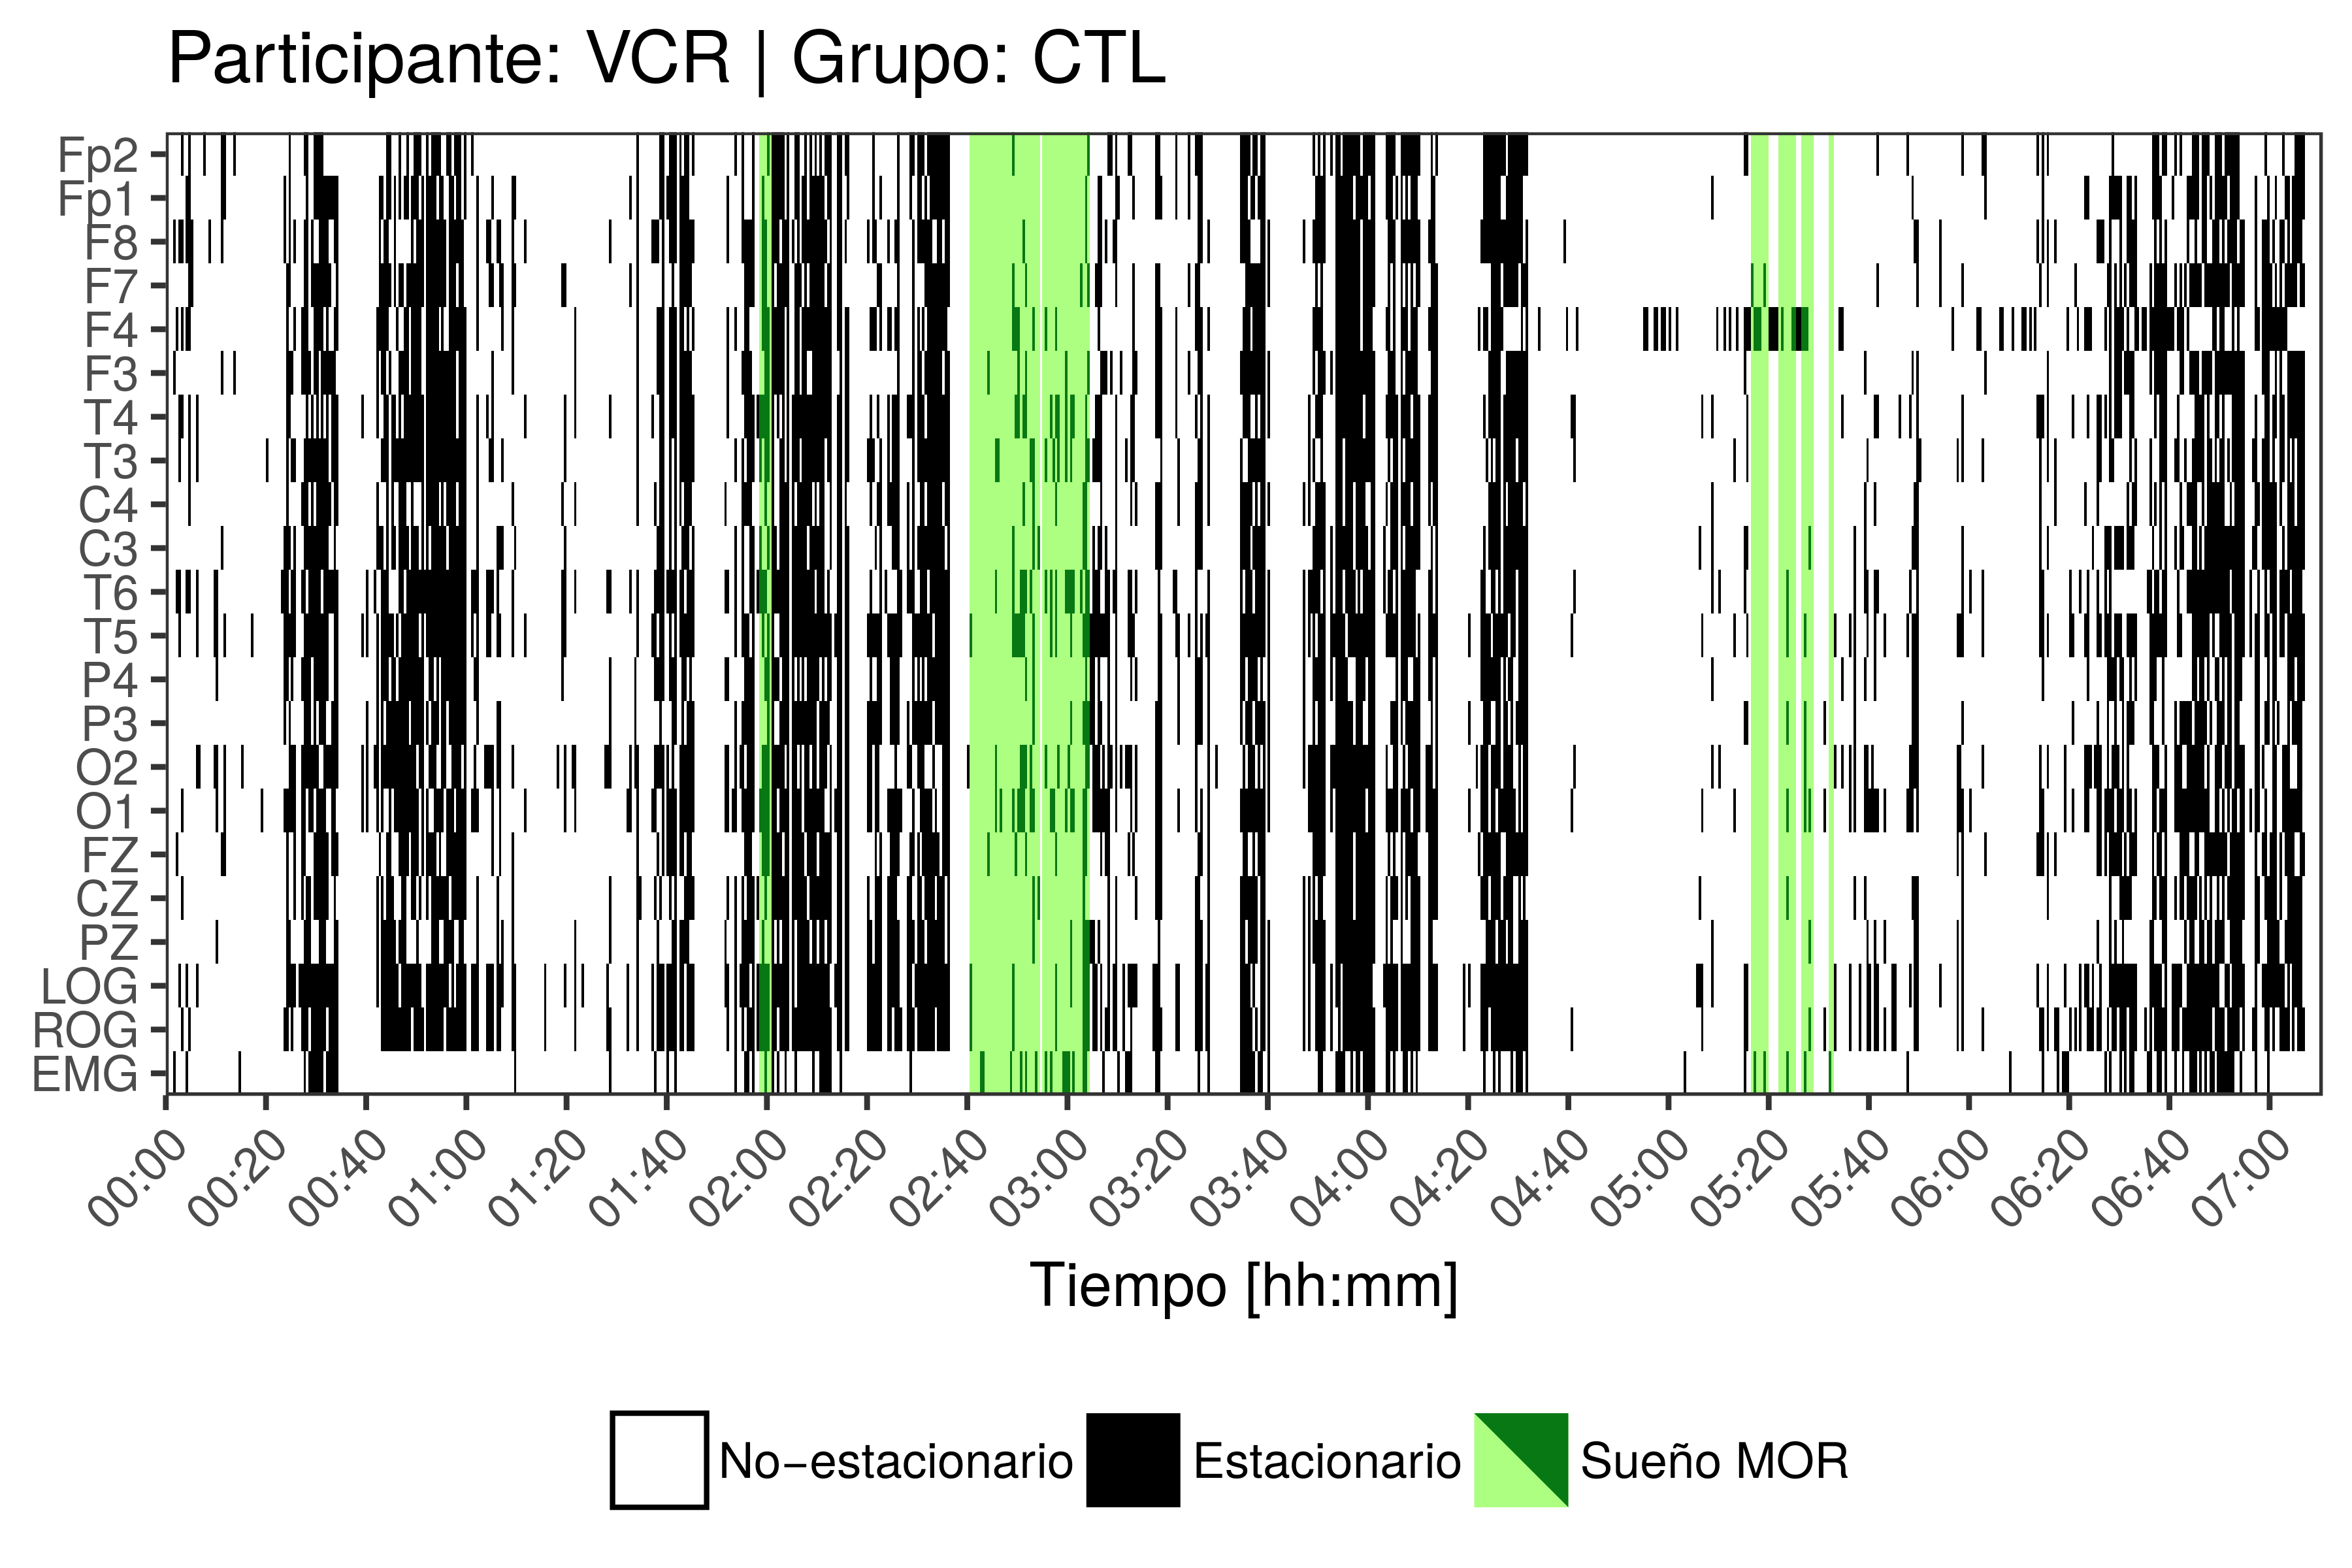
\includegraphics[width=.9\textwidth]
{./img_art_dfa/zoom_noVCR_v2.png} \\
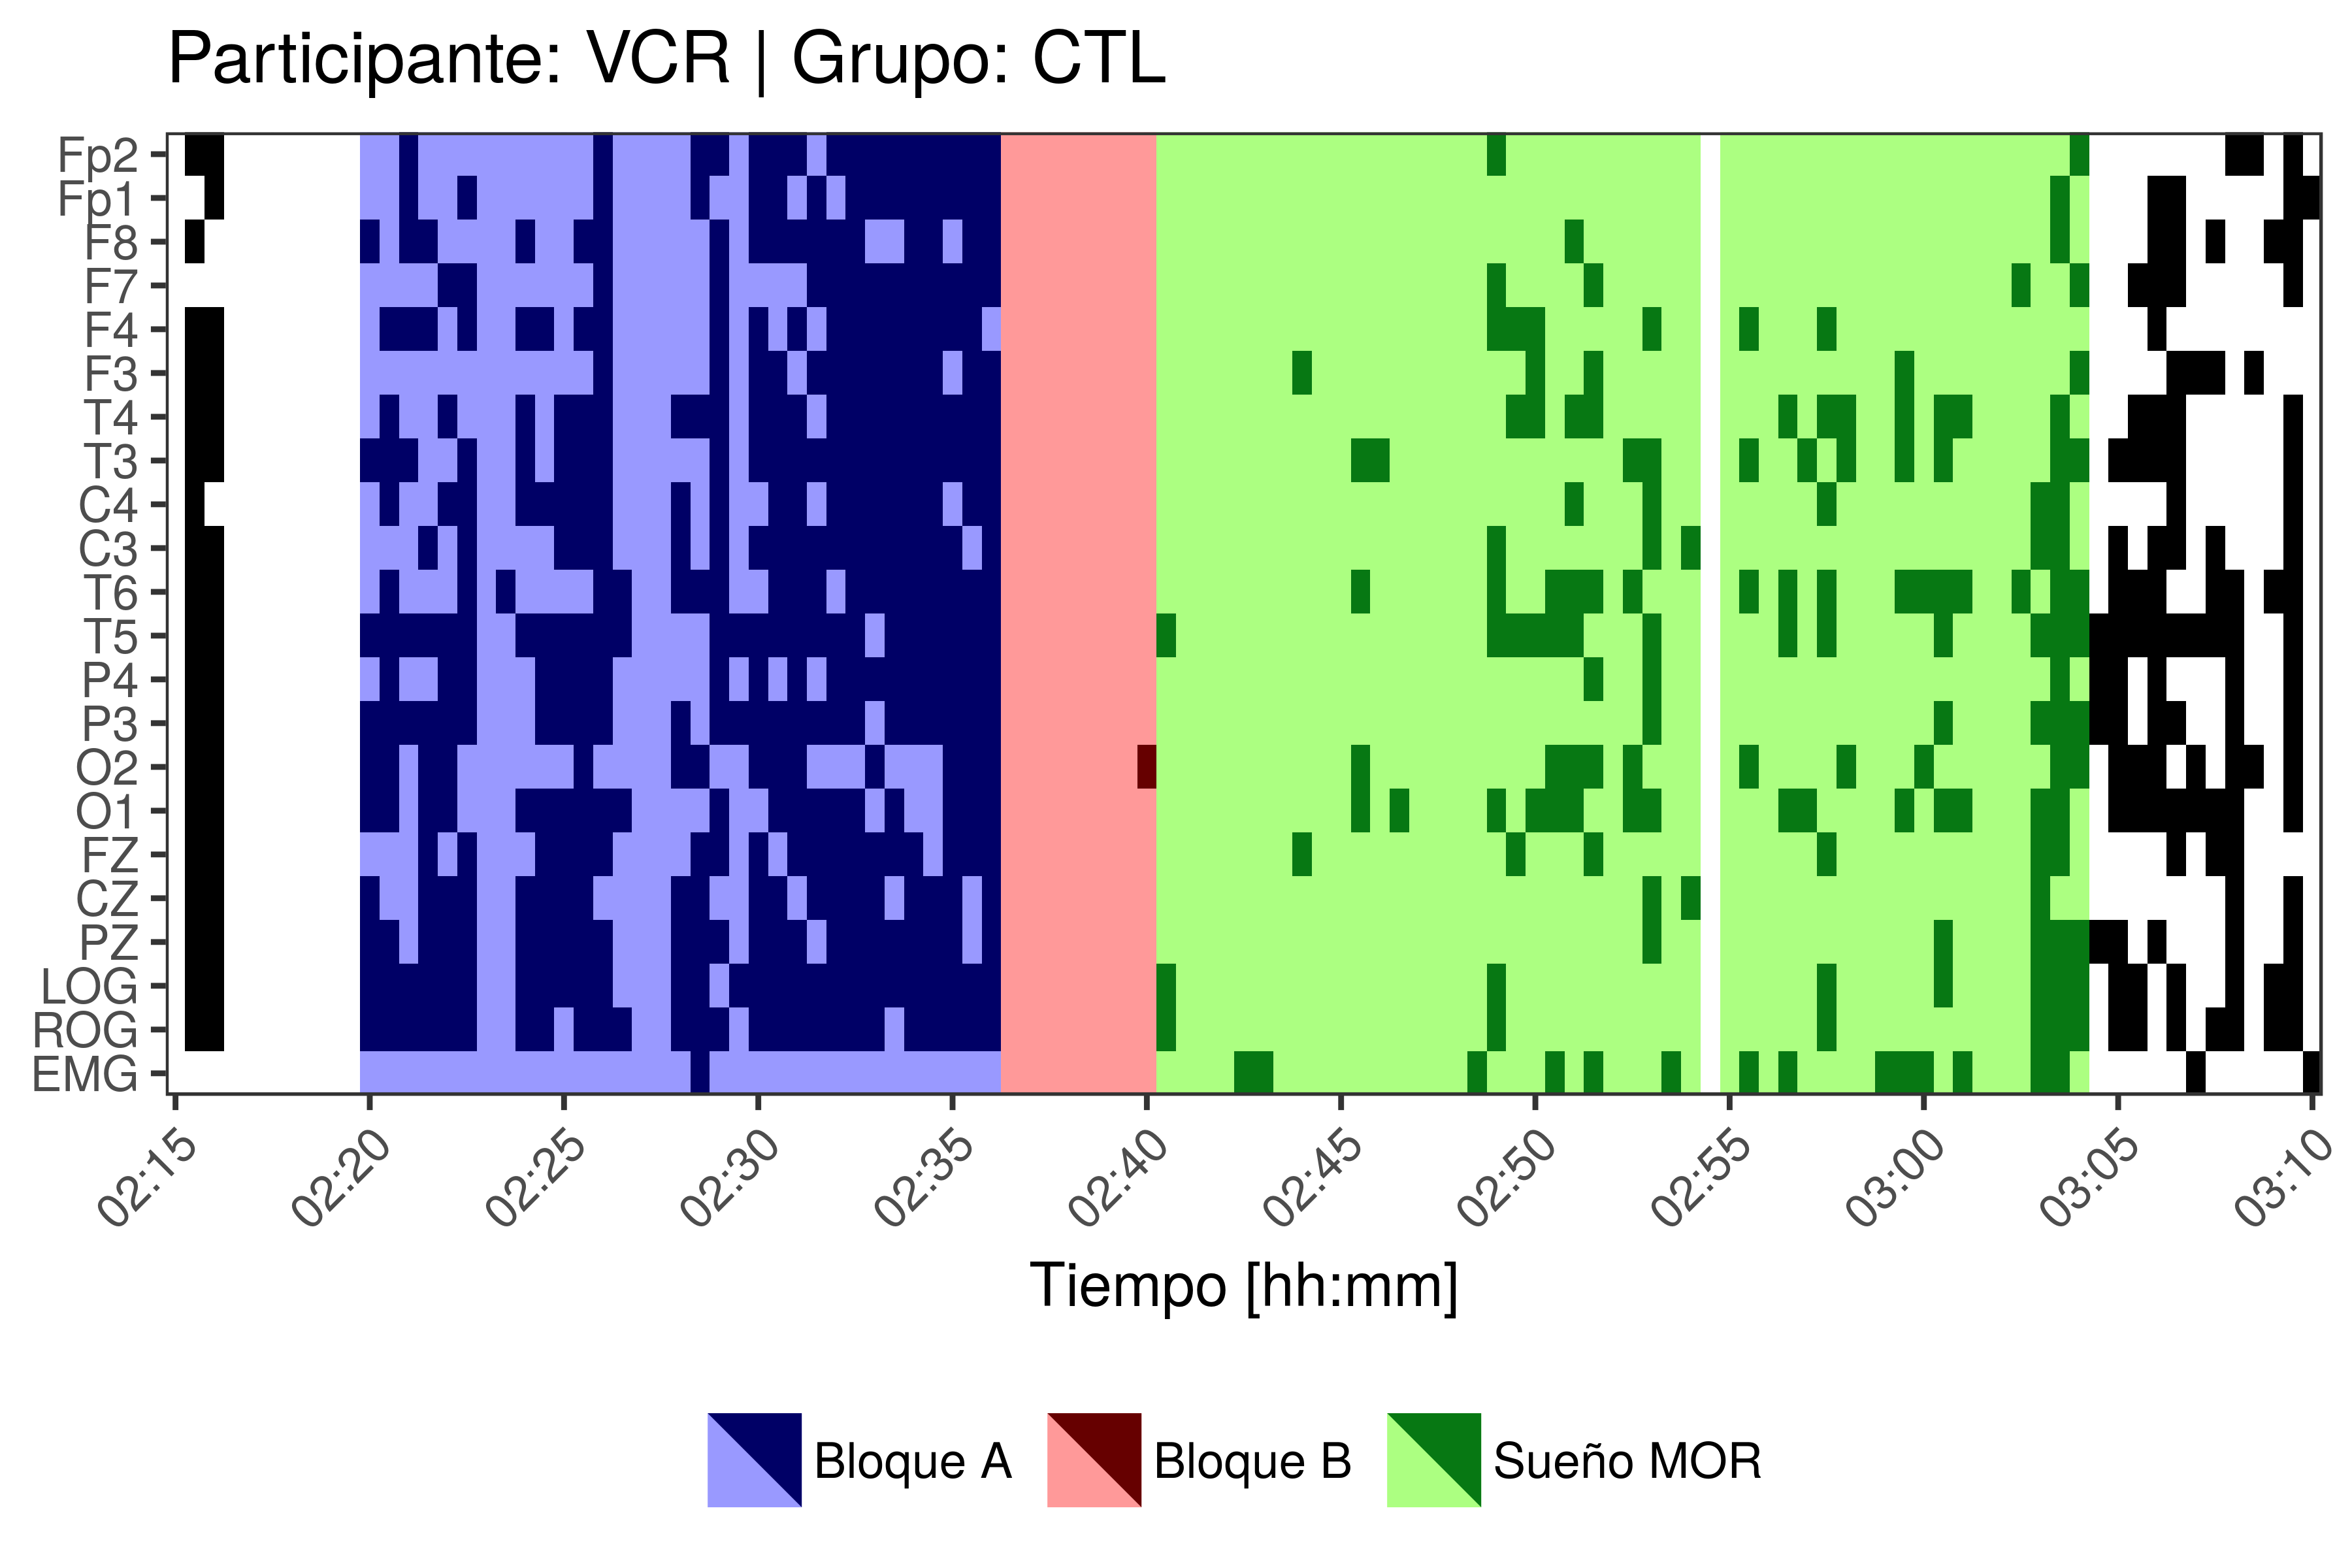
\includegraphics[width=.9\textwidth]
{./img_art_dfa/zoom_siVCR_v2.png}
\caption[Ubicación de épocas estacionarias en el tiempo y patrones emergentes]
{Ubicación de épocas estacionarias en el tiempo y patrones emergentes. \textbf{Arriba:} 
Ubicación de épocas estacionarias en el tiempo.
\textbf{Abajo:} Patrón de bloques relacionado con el sueño MOR}
\label{patroncito}
\end{figure}

%\begin{figure}
%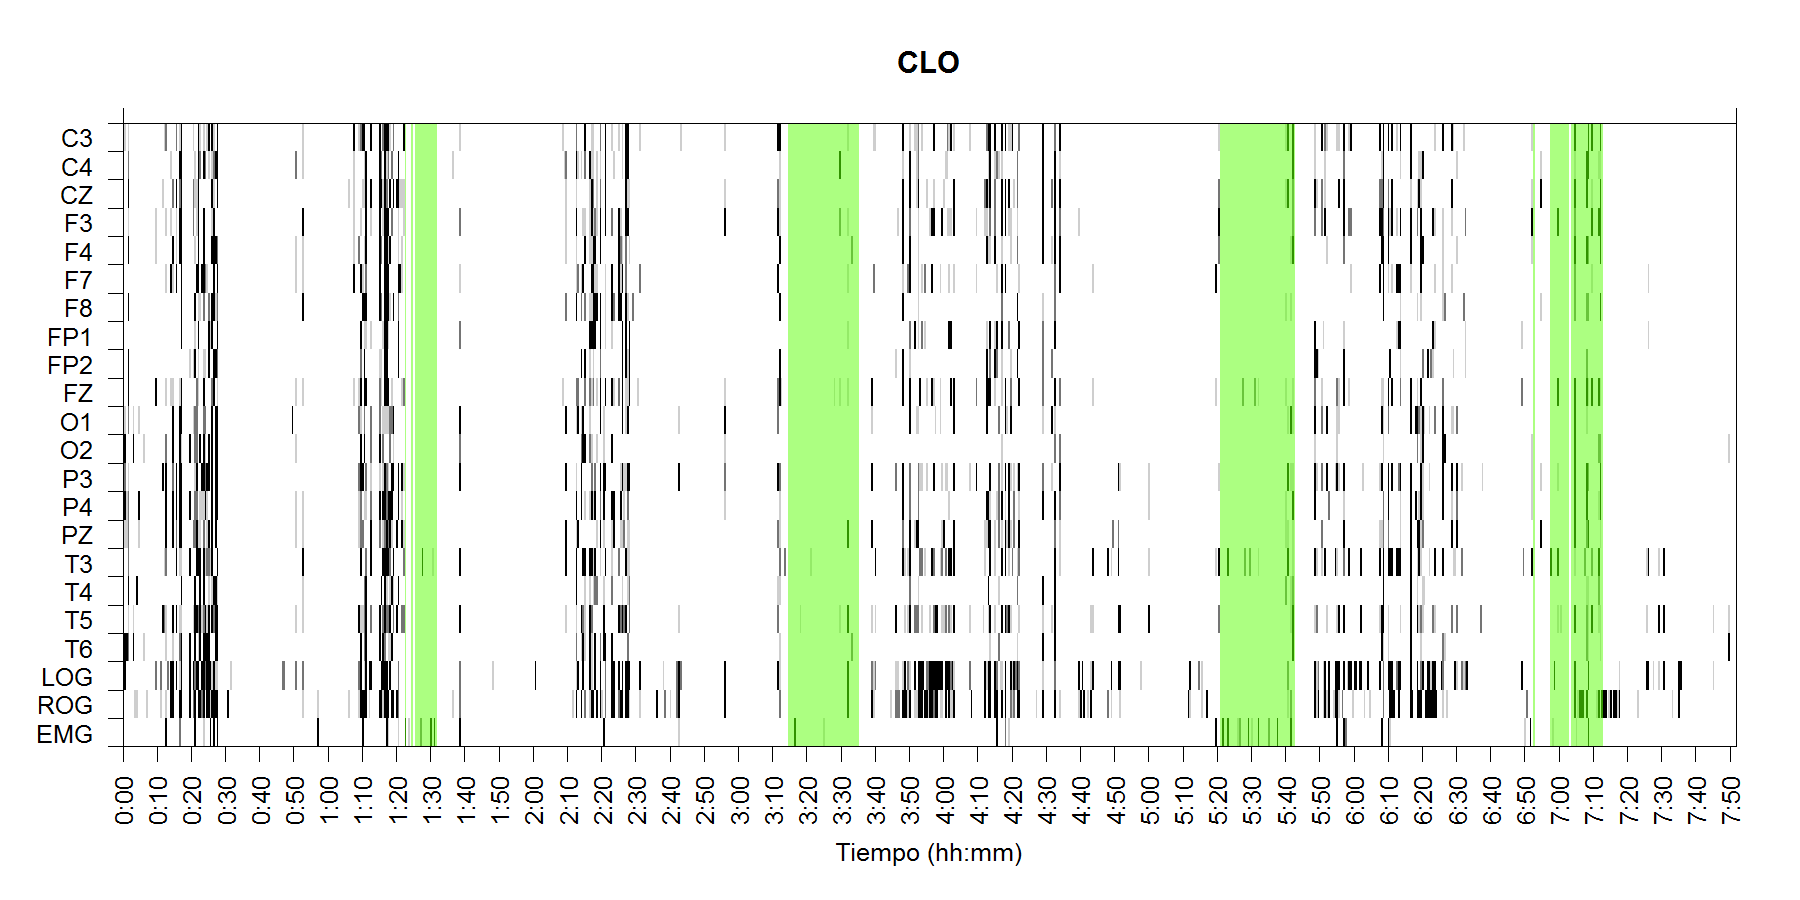
\includegraphics[width=\textwidth]{./img_ejemplos/CLMN10SUE_est.png}
%\caption[Épocas estacionarias ubicadas en el tiempo]{Épocas estacionarias ubicadas en el tiempo. 
%Se ha resaltado en verde las épocas de sueño MOR}
%\label{ejemplo_graf}
%\end{figure}

En otro ámbito,
se replicó la metodología usada por McEwen \cite{McEwen75} para contrastar la afirmación
de que las series de tiempo \textit{suficiente cortas} son estacionarias. 
Este procedimiento consistió en repetir la clasificación de épocas variando el 
tamaño de ventana; los tamaños de ventana se tomaron de la forma $30 \times 2^{n}$ segundos, 
para comparar con el tamaño de época recomendado por la AASM.% (30 segundos).

Usando la clasificación de épocas estacionarias, obtenida para diferentes tamaños de ventana,
se construyeron más gráficos sobre la ubicación de épocas estacionarias en el tiempo. Estos
nuevos
gráficos, como el de la figura \ref{comp_VCR}, refuerzan heurísticamente la hipótesis de que los 
patrones son significativos fisiológicamente. 
%Los gráficos así obtenidos refuerzan la idea de que los patrones no son espurios., y es en base
%a ellos que se obtenidos

\begin{figure}
\centering
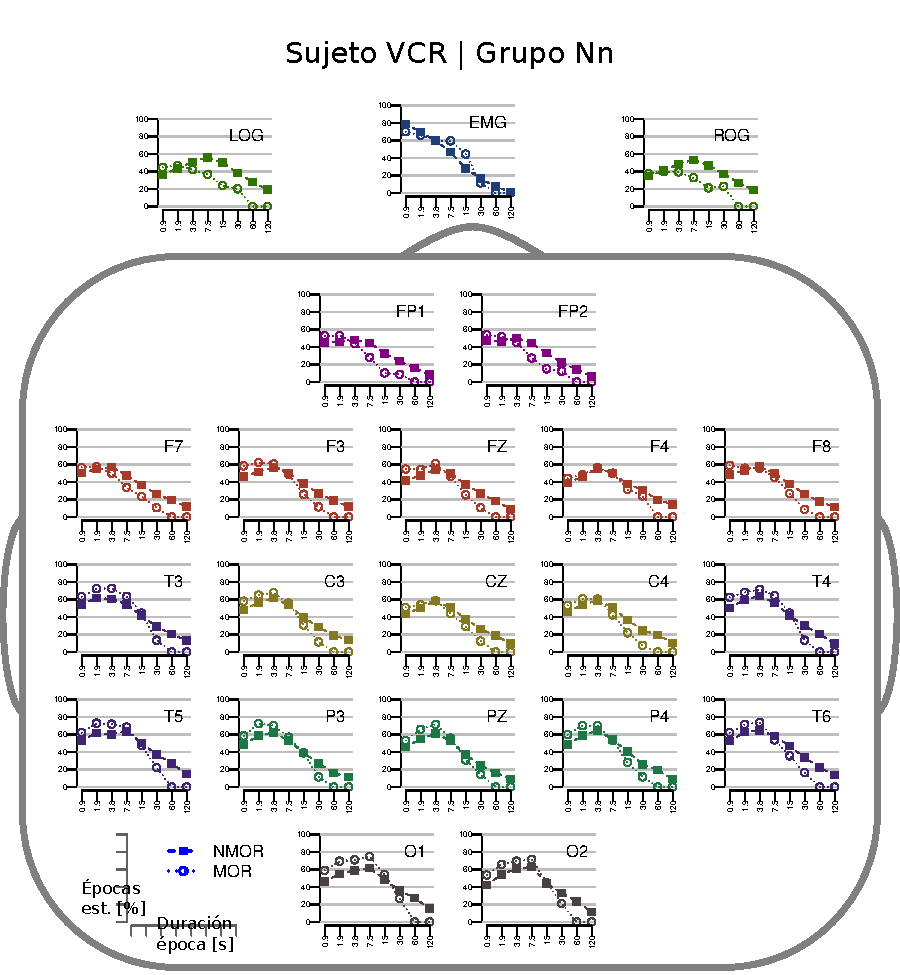
\includegraphics[width=.9\linewidth]{./img_resultados/cabeza_VCR.pdf}
\caption{Cambio en el porcentaje de épocas estacionarias conforme el tamaño de ventana}
\label{cabeza_repoio}
\end{figure}

\begin{figure}
\centering
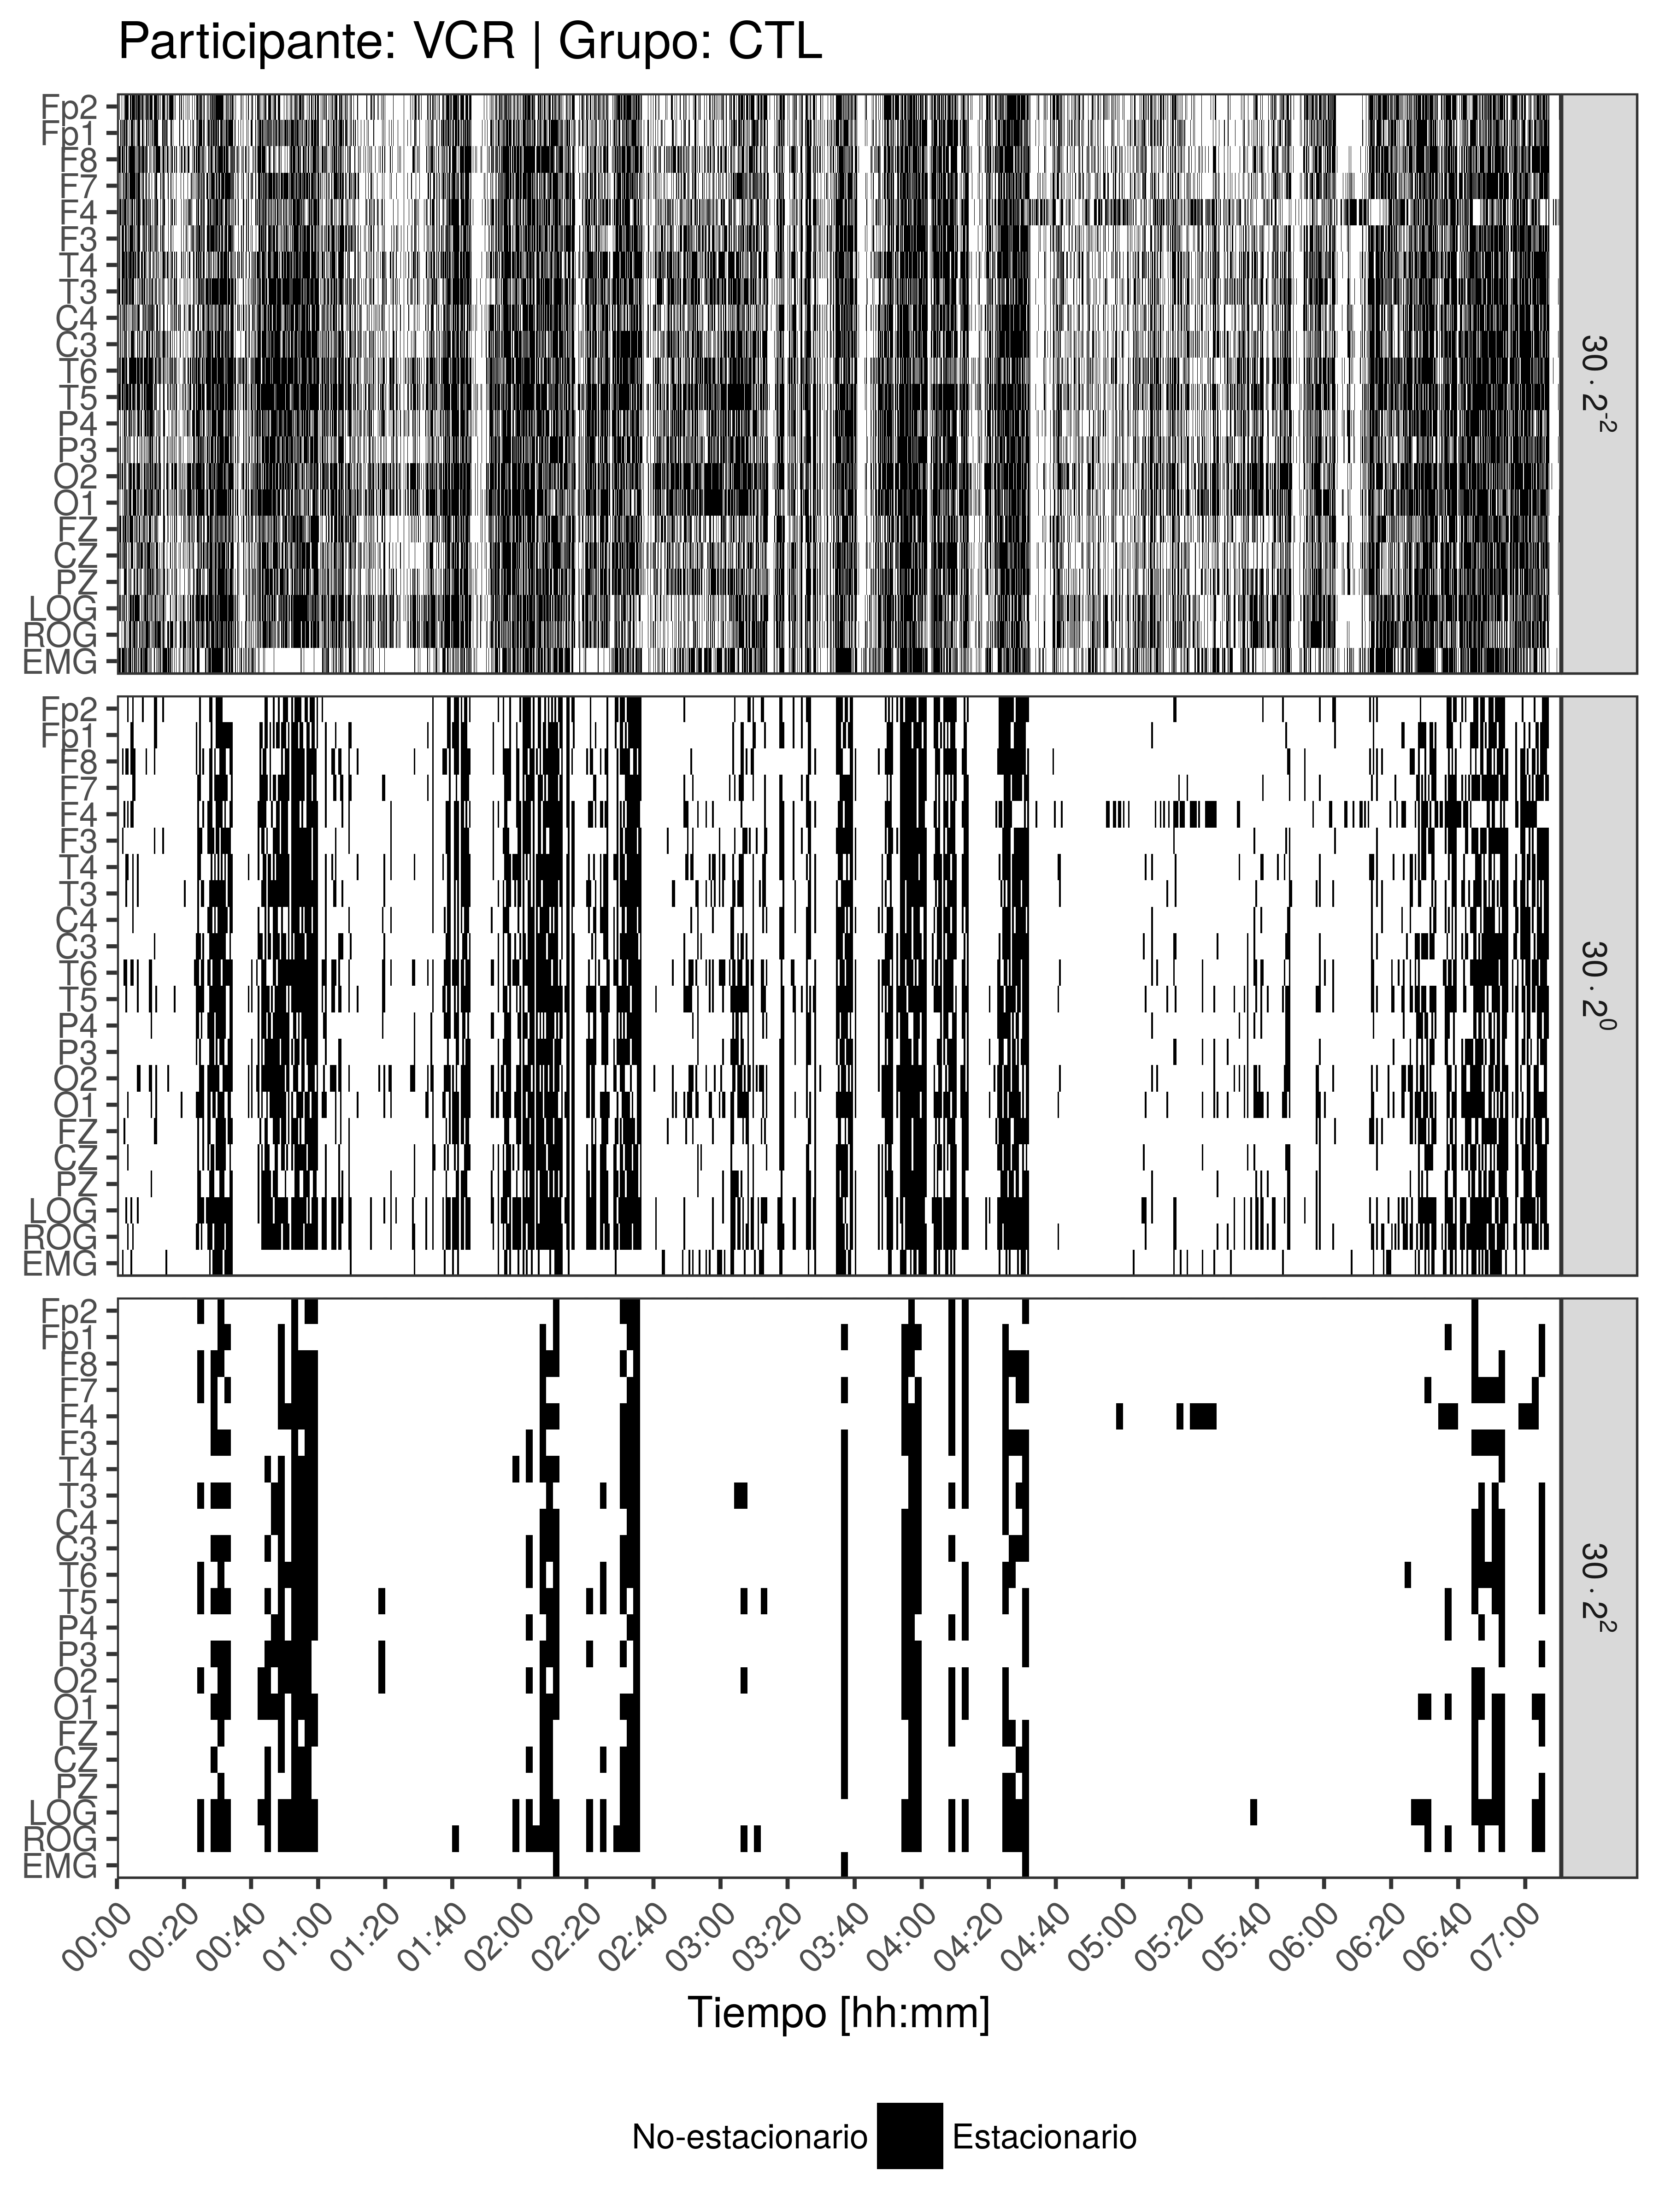
\includegraphics[width=\linewidth]
{./img_art_dfa/VCNNS1_comp_est_.png}
\caption{Distribución en el tiempo de ventanas estacionarias, usando diferentes tamaños
de ventana}
\label{comp_VCR}
\end{figure}

%Todas las clasificaciones se realizaron de forma independiente.
%

%Una práctica común en el análisis de señales electrofisiológicas es el suponer que una serie de 
%tiempo \textit{suficientemente} corta pueda considerarse estacionaria, cuando menos en el sentido
%débil; anteriormente se ha señalado que se trata de un efecto de muestras pequeñas \cite{Melard89},
%y paralelamente se han incorporado a los diseños experimentales motivos para mantener este supuesto
%\cite{Kaiser00}.

Cabe destacar que la aplicación \textit{per se} de la prueba fue efectuada usando el software 
estadístico R \cite{R_citar}. En particular, se utilizó la implementación 
incluida en el paquete \texttt{fractal} \cite{R_fractal} bajo la función \texttt{stationarity}.

\section{Espectro de potencias}

Adicionalmente a la clasificación de épocas como estacionarias, se calculó su espectro de potencia. 
Como una metodología común, se calculó el \textbf{espectro de banda ancha},
es decir, la potencia total y relativa correspondientes a las frecuencias que caracterizan las ondas 
delta, theta, alfa, beta y gamma (ver cuadro \ref{tabla_ondas}).

\begin{figure}
\centering
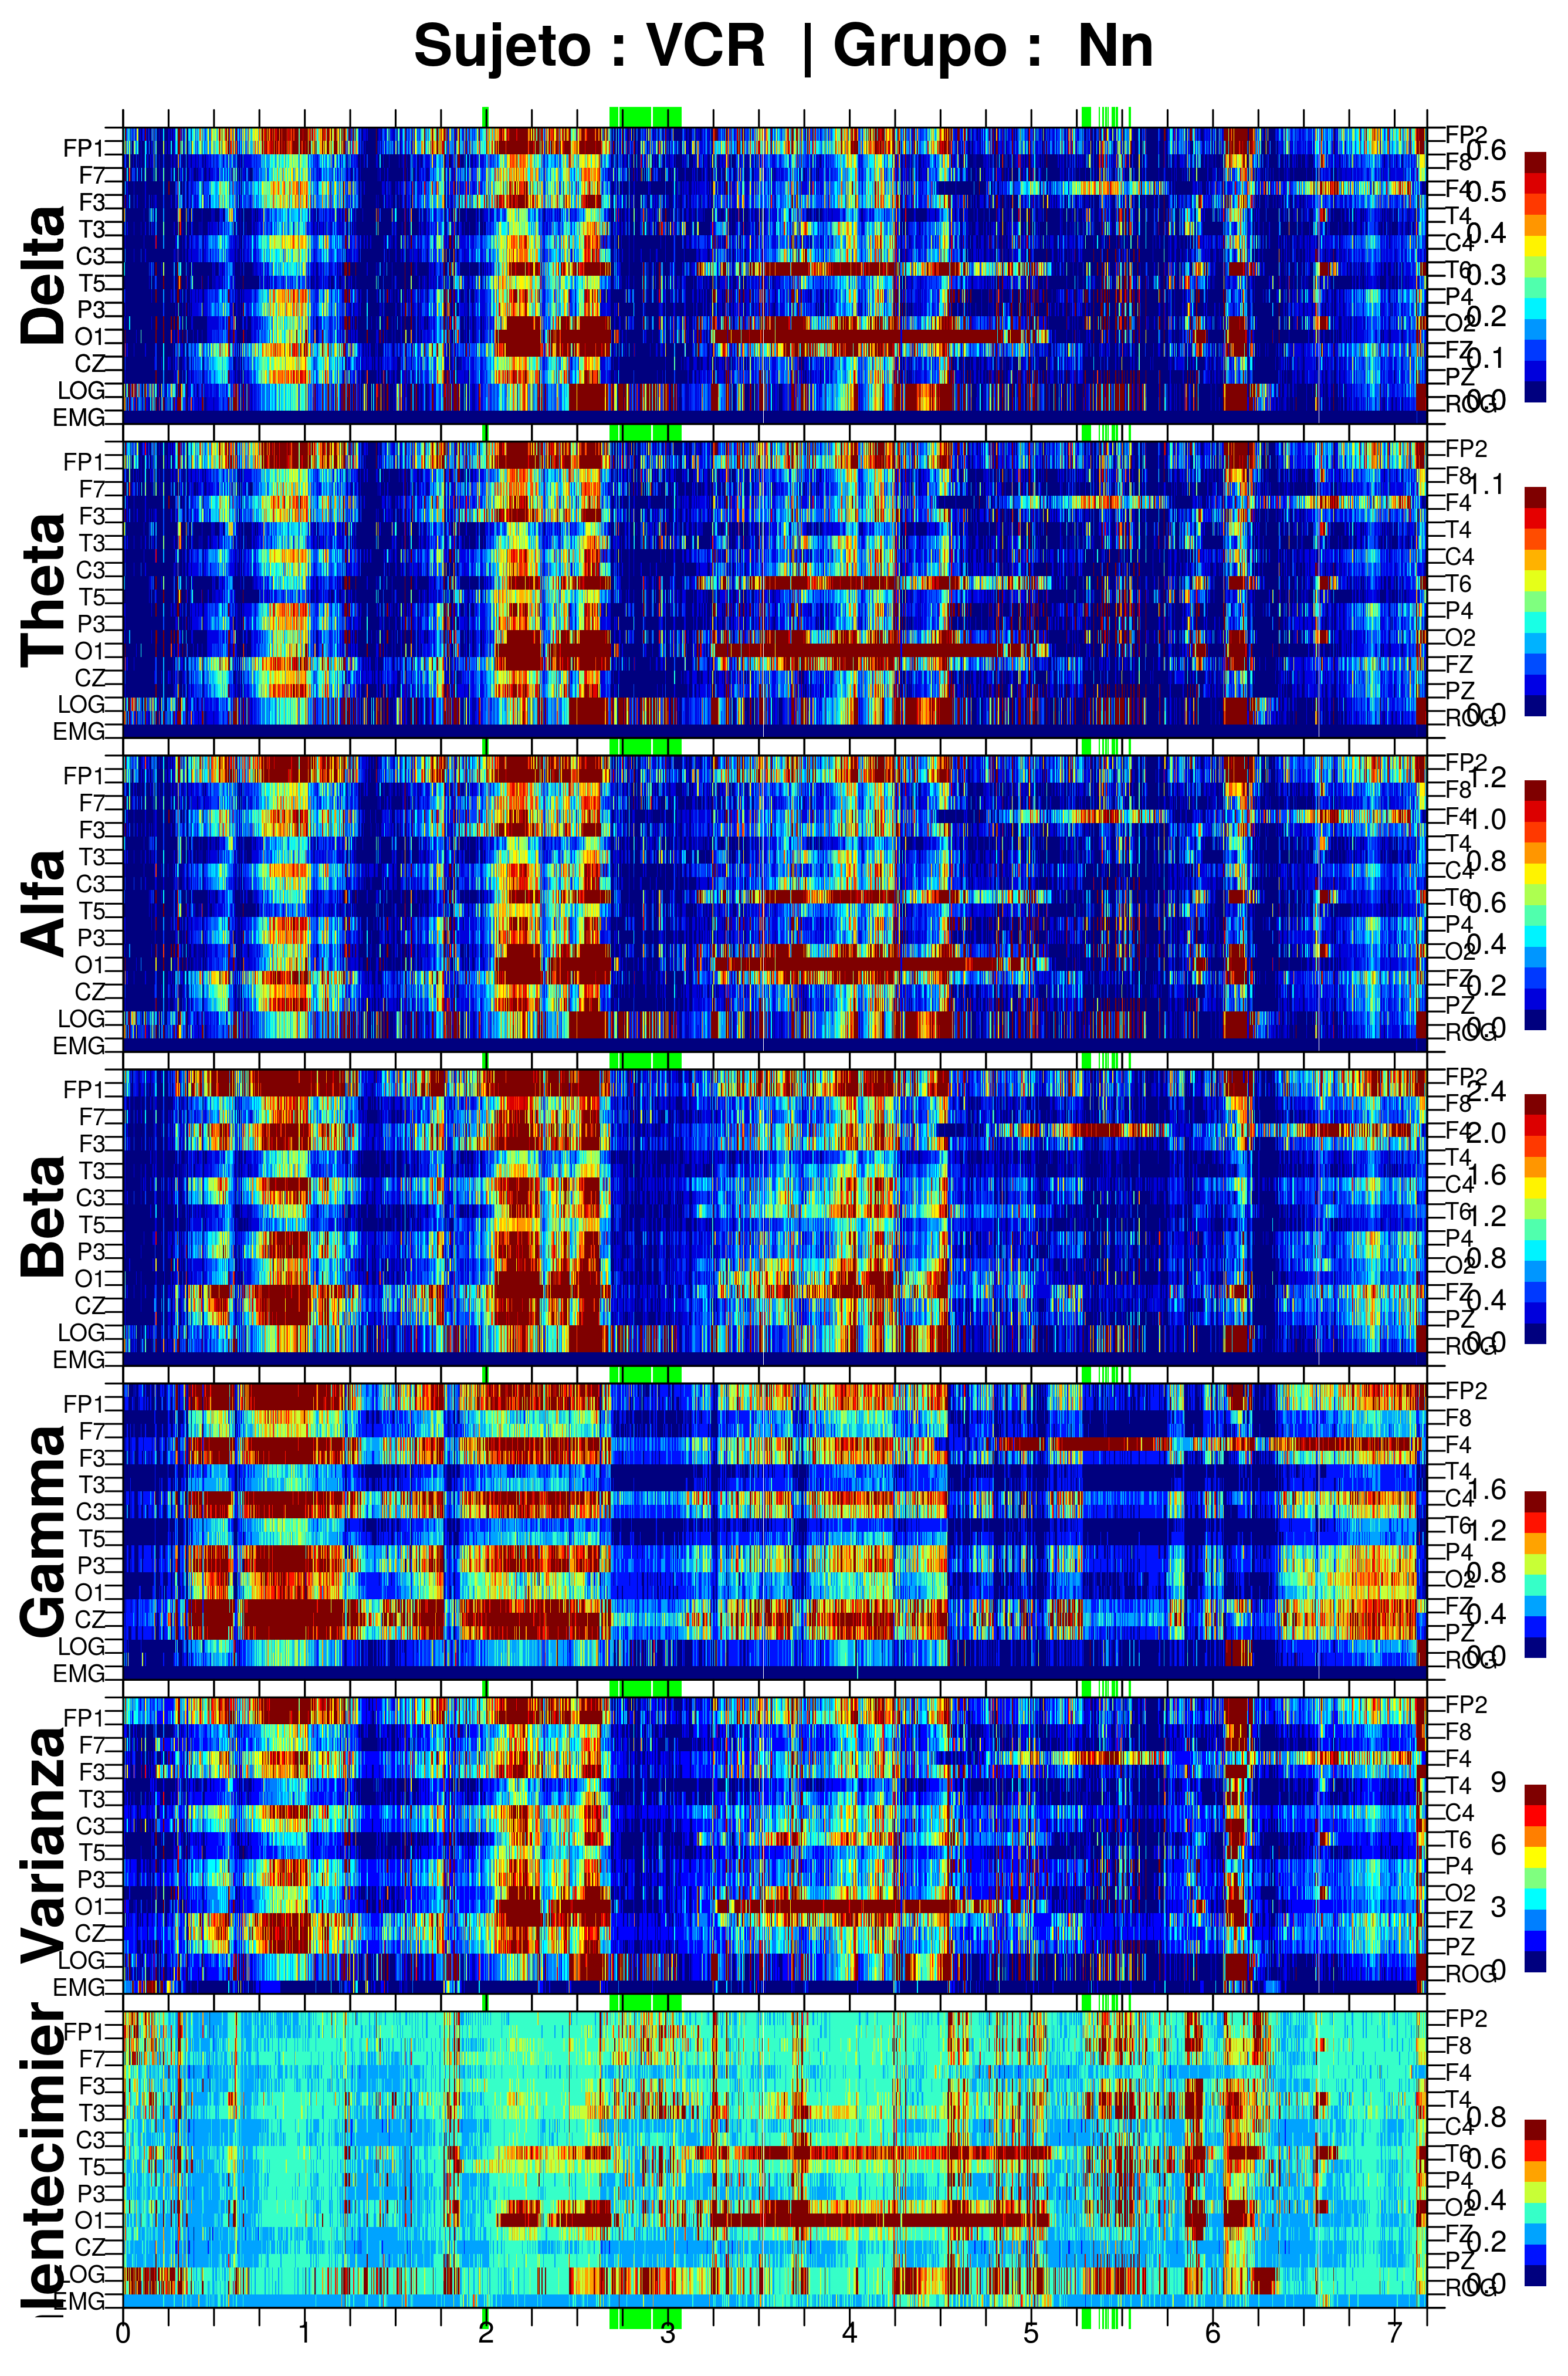
\includegraphics[width=0.8\linewidth]
{./enlentecimiento/VCNNS1_espectral_total.png} 
\caption[Espectro de potencias de banda ancha]{Espectro de potencias de banda ancha (delta, theta
alfa, beta, gamma)}
\end{figure}

Usando los espectros de banda ancha se ha calculado el coeficiente de enlentecimiento \lento, 
definido en la 
expresión \ref{enlentecimiento}, con particular atención al sueño MOR. Esta cantidad
se ha reportado como un posible marcador de deterioro cognitivo leve en adultos mayores 
\cite{Brayet16}.

\begin{equation}
\text{R}_{\text{E}} = \frac{\text{potencia}_{\delta}+\text{potencia}_{\theta}}
{\text{potencia}_{\alpha}+\text{potencia}_{\beta}} =
\frac{\int_{\text 0.5 \hz}^{\text{7 \hz}}h(\omega) d\omega}
{\int_{\text 7 \hz}^{\text{30 \hz}}h(\omega) d\omega}
\label{enlentecimiento}
\end{equation}

El espectro de potencias se ha calculado usado el estimador adaptativo propuesto por
Barbour y Parker \cite{Barbour14}, el cual se encuentra implementado dentro del paquete
\texttt{psd} bajo la función \texttt{pspectrum}.
Se ha usado dicho estimador para garantizar heurísticamente que el espectro de potencias
calculado (1) es independiente del usado para determinar la estacionariedad y (2)
es compatible con la metodología \textit{usual}\footnote{El algoritmo \texttt{psd} 
supone estacionariedad débil; usándolo se espera emular resultados 
obtenidos bajo tal supuesto}.

Como se discute posteriormente, los bloques de épocas estacionarias están relacionados a bloques
cuyo espectro de potencia son distintos. Así mismo son diferentes los coeficientes \lento calculado
para dichos bloques.

%Este estudio se justifica en que la prueba de PSR está basa en el espectro de 
%potencias, luego lo más natural es analizar el espectro de potencias \textit{per se}.

%Debido a que estos \textit{patrones de estacionariedad} se basan primeramente en propiedades del
%espectro de potencias, se graficó el mismo para poder compararlos. Se encontró que, visualmente,
%los patrones en la estacionariedad están relacionados con las ondas Beta.

%Adicionalmente se calculó por cada época el \textit{coeficiente de enlentecimiento}, 
%$R_\text{lento}$, el cual se encuentra asociado con el deterioro cognitivo leve \cite{Brayet16}; 
%esta cantidad se define como

%%%%%%%%%%%%%%%%%%%%%%%%%%%%%%%%%%%%%%%%%%%%%%%%%%%%%%%%%%%%%%%%%%%%%%%%%%%%%%%%%%%%%%%%%%%%%%%%%%%
%%%%%%%%%%%%%%%%%%%%%%%%%%%%%%%%%%%%%%%%%%%%%%%%%%%%%%%%%%%%%%%%%%%%%%%%%%%%%%%%%%%%%%%%%%%%%%%%%%%
%%%%%%%%%%%%%%%%%%%%%%%%%%%%%%%%%%%%%%%%%%%%%%%%%%%%%%%%%%%%%%%%%%%%%%%%%%%%%%%%%%%%%%%%%%%%%%%%%%%
%%%%%%%%%%%%%%%%%%%%%%%%%%%%%%%%%%%%%%%%%%%%%%%%%%%%%%%%%%%%%%%%%%%%%%%%%%%%%%%%%%%%%%%%%%%%%%%%%%%